\chapter{Resultados}
\label{cap:resultados}

Esta seção apresenta os resultados experimentais obtidos com a aplicação da metodologia descrita na Seção~\ref{sec:method}. O objetivo é validar as abordagens propostas e analisar o comportamento do modelo sob diferentes condições. Inicialmente, detalham-se o ambiente computacional utilizado e a seleção dos hiperparâmetros para o treinamento do modelo \textit{baseline}. Na sequência, investiga-se o impacto da etapa de remoção de ruído e das diferentes formulações da função de perda no desempenho preditivo. Por fim, conduz-se um estudo comparativo abrangente entre diferentes arquiteturas da família EfficientNet, avaliando o compromisso entre custo computacional e eficácia.

\section{Ambiente Experimental}

Os experimentos foram conduzidos em uma estação de trabalho Linux equipada com um processador AMD Ryzen 5 5600X, 32 GB de memória RAM DDR4 (3200 MHz) e uma GPU NVIDIA GeForce RTX 3060 (12 GB de VRAM), dedicada à aceleração do treinamento de modelos de aprendizado profundo.

O desenvolvimento foi realizado em Python, utilizando o \textit{framework} PyTorch integrado ao CUDA 12.8. Para o processamento das imagens histopatológicas, empregou-se a biblioteca OpenSlide para a leitura e a extração de patches. O cálculo das métricas de avaliação foi realizado com o scikit-learn, enquanto as análises visuais foram geradas com a biblioteca Matplotlib.

\section{Configuração de Hiperparâmetros}

A etapa inicial da experimentação consistiu em uma \textit{grid search} para identificar a configuração de hiperparâmetros que maximizasse a convergência e a capacidade de generalização do modelo \textit{baseline}, mitigando o risco de \textit{overfitting}. Os valores explorados e a configuração final selecionada estão consolidados na Tabela~\ref{tab:hiperparametros_gridsearch}. Essa configuração ótima foi estabelecida como padrão e mantida constante nos experimentos subsequentes, a fim de garantir a comparabilidade dos resultados.

A taxa de aprendizado inicial fixada em $3\times10^{-4}$, operando em conjunto com o otimizador Adam, proporcionou a melhor estabilidade durante a minimização da função de perda (BCE). No processo de \textit{fine-tuning}, adotou-se a estratégia de descongelamento dos últimos 150 parâmetros/camadas treináveis do modelo, o que apresentou o melhor equilíbrio.. Aliada a isso, uma camada de \textit{dropout} com probabilidade de retenção de 0,4 demonstrou ser a regularização mais eficaz.

O tamanho do batch foi limitado a duas amostras devido às limitações de memória da GPU. Para mitigar as flutuações na atualização dos gradientes decorrentes do lote reduzido, configurou-se o treinamento para até 50 épocas, adotando-se um critério de \textit{early stopping} com tolerância de 7 épocas sem melhoria na métrica de validação.

\begin{table}[htb]
	\centering
	\resizebox{\linewidth}{!}{
		\begin{tabular}{lll}
			\toprule
			\textbf{Parâmetro} & \textbf{Valores avaliados} & \textbf{Valor selecionado} \\
			\midrule
			Taxa de aprendizado & $3\times10^{-4}$, $3\times10^{-3}$, $1\times10^{-4}$ & $3\times10^{-4}$ \\
			Número de épocas & 50 & 50 \\
			Camadas descongeladas (\textit{fine-tuning}) & 100, 150 & 150 \\
			\textit{Dropout} & 0.4, 0.5, 0.6 & 0.4 \\
			Tamanho do lote (\textit{batch size}) & 2 & 2 \\
			Função de perda & BCE & BCE \\
			Otimizador & Adam & Adam \\
			\bottomrule
		\end{tabular}
	}
	\caption{Hiperparâmetros avaliados e configuração selecionada para os experimentos.}
	\label{tab:hiperparametros_gridsearch}
\end{table}

\section{Impacto da Filtragem de Ruído e Funções de Perda}

Com o conjunto ideal de hiperparâmetros definido, procedeu-se ao treinamento do modelo \textit{baseline} com a arquitetura EfficientNet-B0 e a função de perda BCE. Este modelo alcançou uma acurácia de 0,592 e um coeficiente Kappa de 0.826. No contexto da classificação de graus ISUP em biópsias de próstata, este valor de Kappa é considerado altamente satisfatório e competitivo. A literatura médica aponta uma expressiva variabilidade interobservador na graduação histopatológica \cite{Ozkan2016Gleason, cinar2025assessment}. Enquanto uropatologistas experientes frequentemente alcançam valores de Kappa entre 0.43 e 0.68 \cite{Ozkan2016Gleason} , avaliações recentes focadas especificamente nos graus ISUP relatam níveis de concordância mínimos entre patologistas, com Kappa na faixa de 0.31 \cite{cinar2025assessment}. Dessa forma, o baseline obtido demonstra um nível de concordância que supera consideravelmente a variabilidade humana relatada. Ademais, os resultados indicam que, mesmo com uma acurácia moderada (59,2\%), os erros de predição do modelo concentram-se em graus ISUP adjacentes, minimizando penalidades clínicas graves.

A etapa de filtragem baseada em entropia permitiu identificar um subconjunto de 903 amostras, correspondentes aos 10\% com maior incerteza entre as predições dos modelos EfficientNet-B0, B1, B2 e B3. A análise desse subconjunto revelou características que demonstram grande dificuldade para os modelos, incluindo alta entropia média ($0.3851 \pm 0.0638$), grande variabilidade nas predições ($1.1188 \pm 0.8943$) e baixa concordância entre as arquiteturas avaliadas. Observou-se que apenas 6,2\% das amostras apresentaram consenso entre os quatro modelos. Além disso, em 58\% das instâncias classificadas como \textit{hard samples}, nenhum dos modelos foi capaz de realizar a predição correta, esses dados sustentam a hipótese de que a entropia pode atuar como um indicador eficaz para a identificação de exemplos difíceis ou inconsistentes.

Ademais, a análise da distribuição dessas \textit{hard samples} revelou que a incerteza das redes não é homogênea entre as classes, mas fortemente associada à severidade da lesão. Aproximadamente 81,7\% das imagens de alta entropia concentram-se nos graus ISUP 3, 4 e 5. Esse comportamento reflete a complexidade morfológica e a maior heterogeneidade visual inerentes aos tumores mais agressivos, o que naturalmente impõe um desafio maior para a extração de características convolucionais.

A partir desse subconjunto de \textit{hard samples}, foram investigados diferentes cenários de remoção de dados potencialmente ruidosos durante o treinamento. Os resultados indicaram que a remoção parcial dessas amostras contribuiu para a melhoria do desempenho do modelo. Na Figura \ref{fig:acckappa}, observa-se que a exclusão de aproximadamente 20\% das \textit{hard samples} proporcionou o melhor equilíbrio entre a redução do ruído e a preservação da diversidade do conjunto de treinamento, sugerindo que uma filtragem moderada pode favorecer a capacidade de generalização do modelo.

\begin{figure}[H]
	\centering
	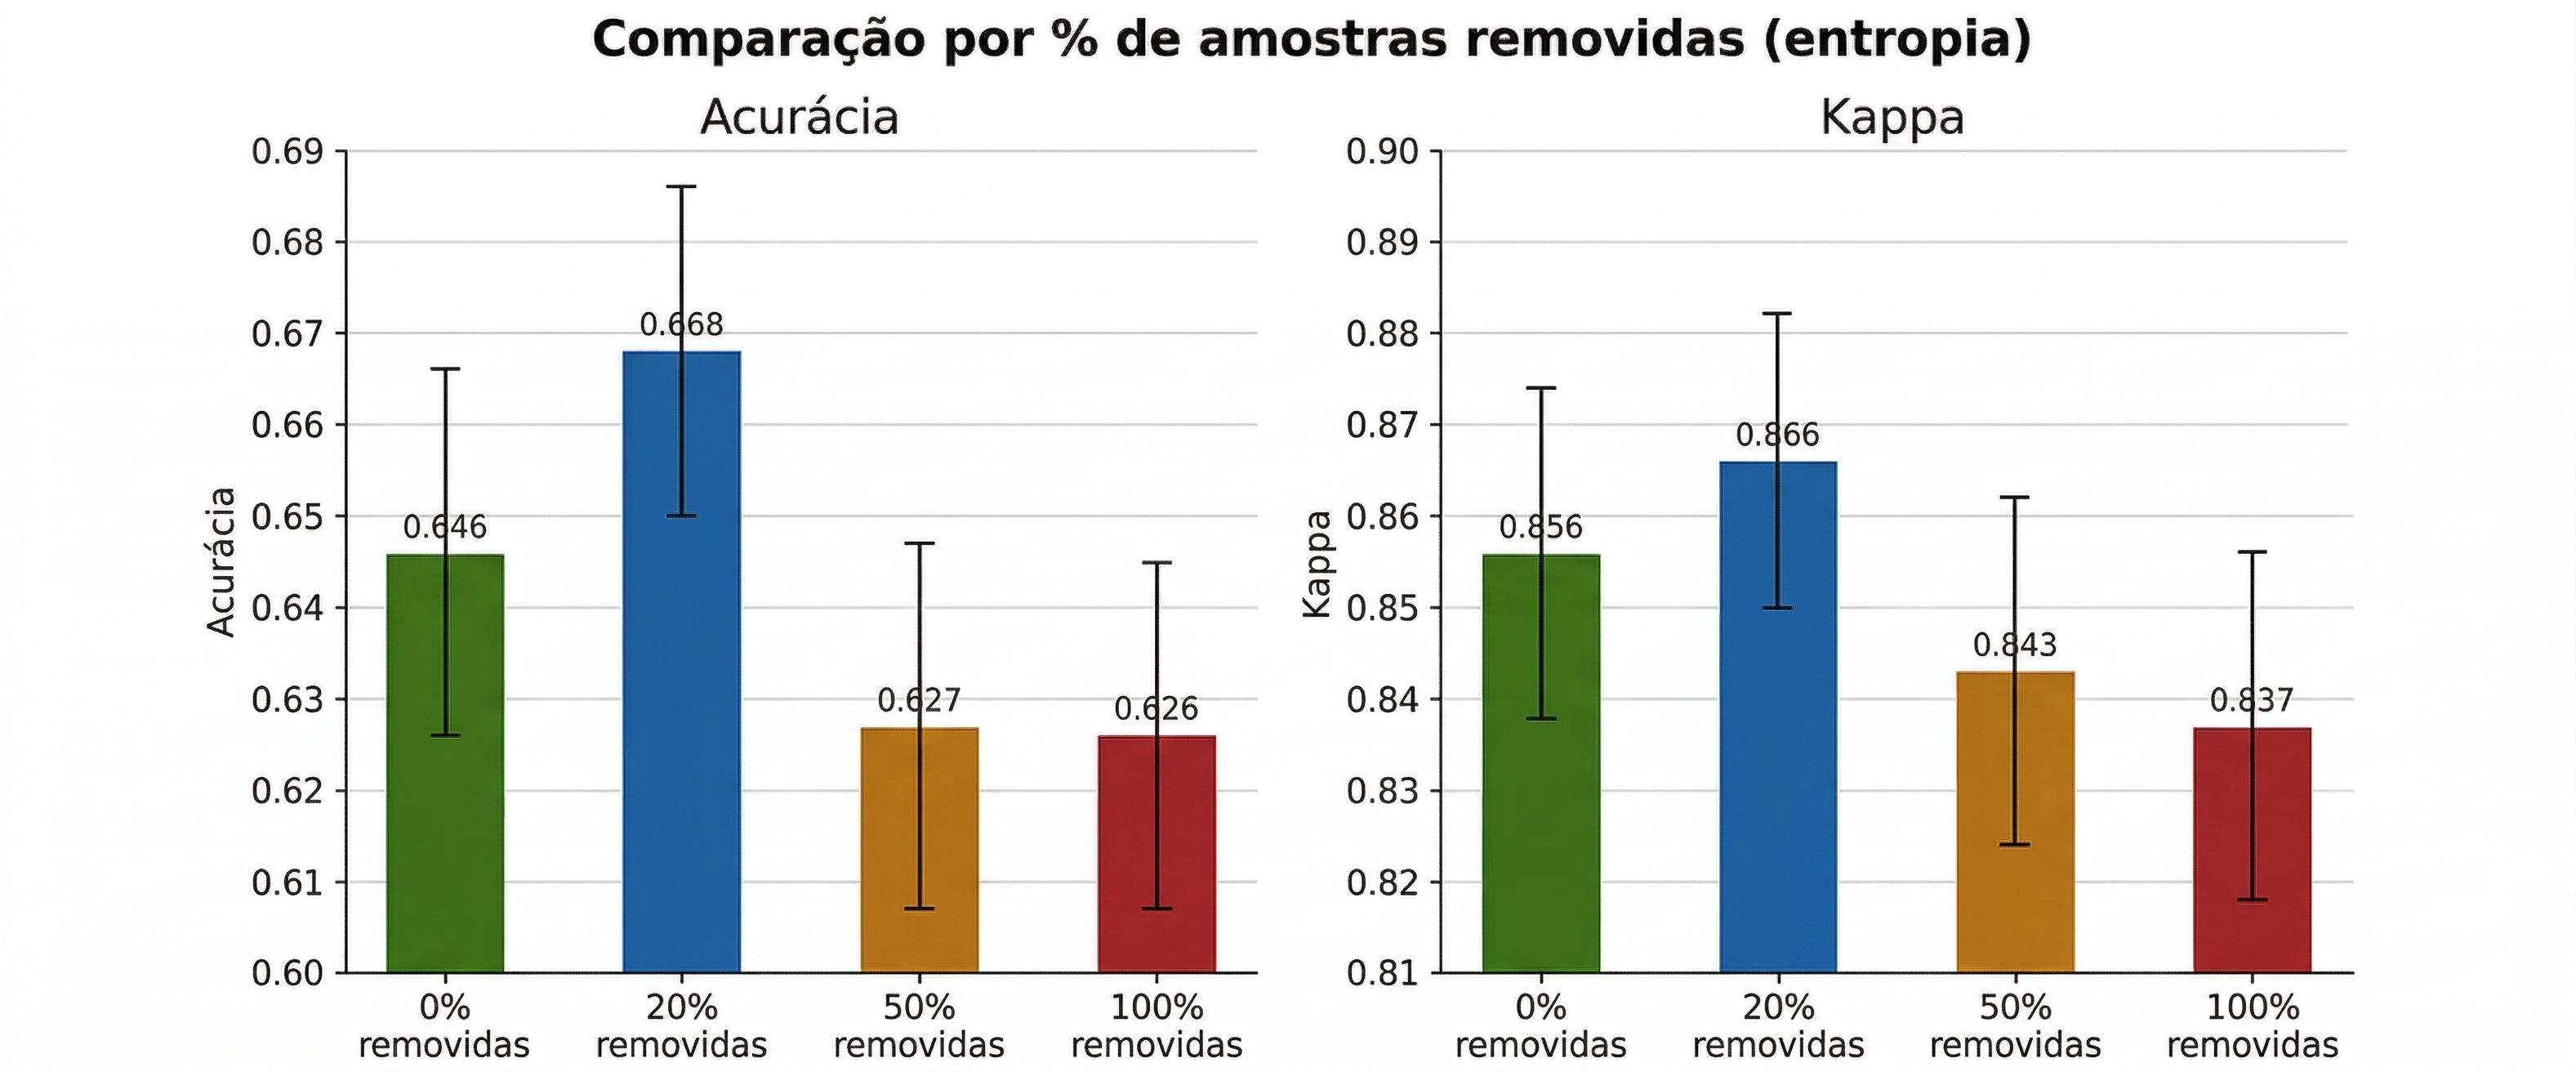
\includegraphics[width=1\linewidth]{figuras/acc_kappa.png}
	\caption{Desempenho com diferentes limiares de remoção de ruído sobre os \textit{hard samples}}
	\label{fig:acckappa}
\end{figure}


A Figura~\ref{fig:maxentropy} apresenta um exemplo de imagem identificada pelo método como uma amostra com elevado grau de incerteza na predição. Ao analisar os resultados obtidos pelos modelos, observa-se que o rótulo verdadeiro da imagem corresponde à classe ISUP 2. Entretanto, durante o processo de inferência, o modelo EfficientNet-B0 a classificou como ISUP 3, enquanto os modelos EfficientNet-B1, B2 e B3 a classificaram como ISUP 1. Embora essas discrepâncias não representem erros clinicamente graves, a análise realizada nesta etapa prioriza o nível de incerteza associado às decisões dos modelos. Para essa imagem específica, o valor médio de entropia calculado foi de 0,59, considerado alto. Esse exemplo ilustra como o método é capaz de identificar casos potencialmente ruidosos; nessa imagem em específico, ficam evidentes as anotações de caneta. A eficácia dessa estratégia de filtragem torna-se mais evidente ao analisar os resultados apresentados na Tabela~\ref{tab:impacto_loss_expandido}. Observa-se que a aplicação da remoção de ruído elevou o $\kappa_{\text{quad}}$ do valor de $0.826$ no modelo \textit{baseline} para $0.833$. O impacto na acurácia foi ainda mais significativo, passando de $0.592$ para $0.638$, o que representa um ganho absoluto de aproximadamente 4,6 pontos percentuais. Esses resultados indicam que a remoção de uma parcela das amostras altamente incertas melhora a capacidade de generalização do modelo.


\begin{figure}[H]
	\centering
	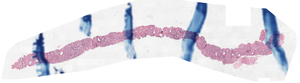
\includegraphics[width=0.7\linewidth]{figuras/max_entropy.png}
	\caption{Imagem identificada como ruído pelo método de filtragem}
	\label{fig:maxentropy}
\end{figure}

A substituição da função de perda BCE pela formulação ordinal elevou o desempenho global do modelo para $0.851$, embora tenha ocorrido uma leve redução na acurácia. Esse resultado sugere que a inclusão do fator ordinal promove uma redistribuição das predições incorretas, reduzindo os erros entre classes distantes e concentrando as confusões entre classes adjacentes. Em problemas de classificação ordinal, como no sistema de graduação ISUP, esse comportamento é desejável, pois discrepâncias entre classes vizinhas têm menor impacto clínico do que erros entre graus mais distantes. Esse comportamento pode ser observado na Figura \ref{fig:confusionmatricesbaseline}, que apresenta as matrizes de confusão normalizadas dos modelos treinados com BCE e com a função de perda ordinal. Nota-se que o modelo com perda ordinal concentra os erros principalmente entre classes adjacentes, enquanto o modelo treinado com BCE apresenta maior dispersão entre classes mais distantes.

\begin{figure}[htb]
	\centering
	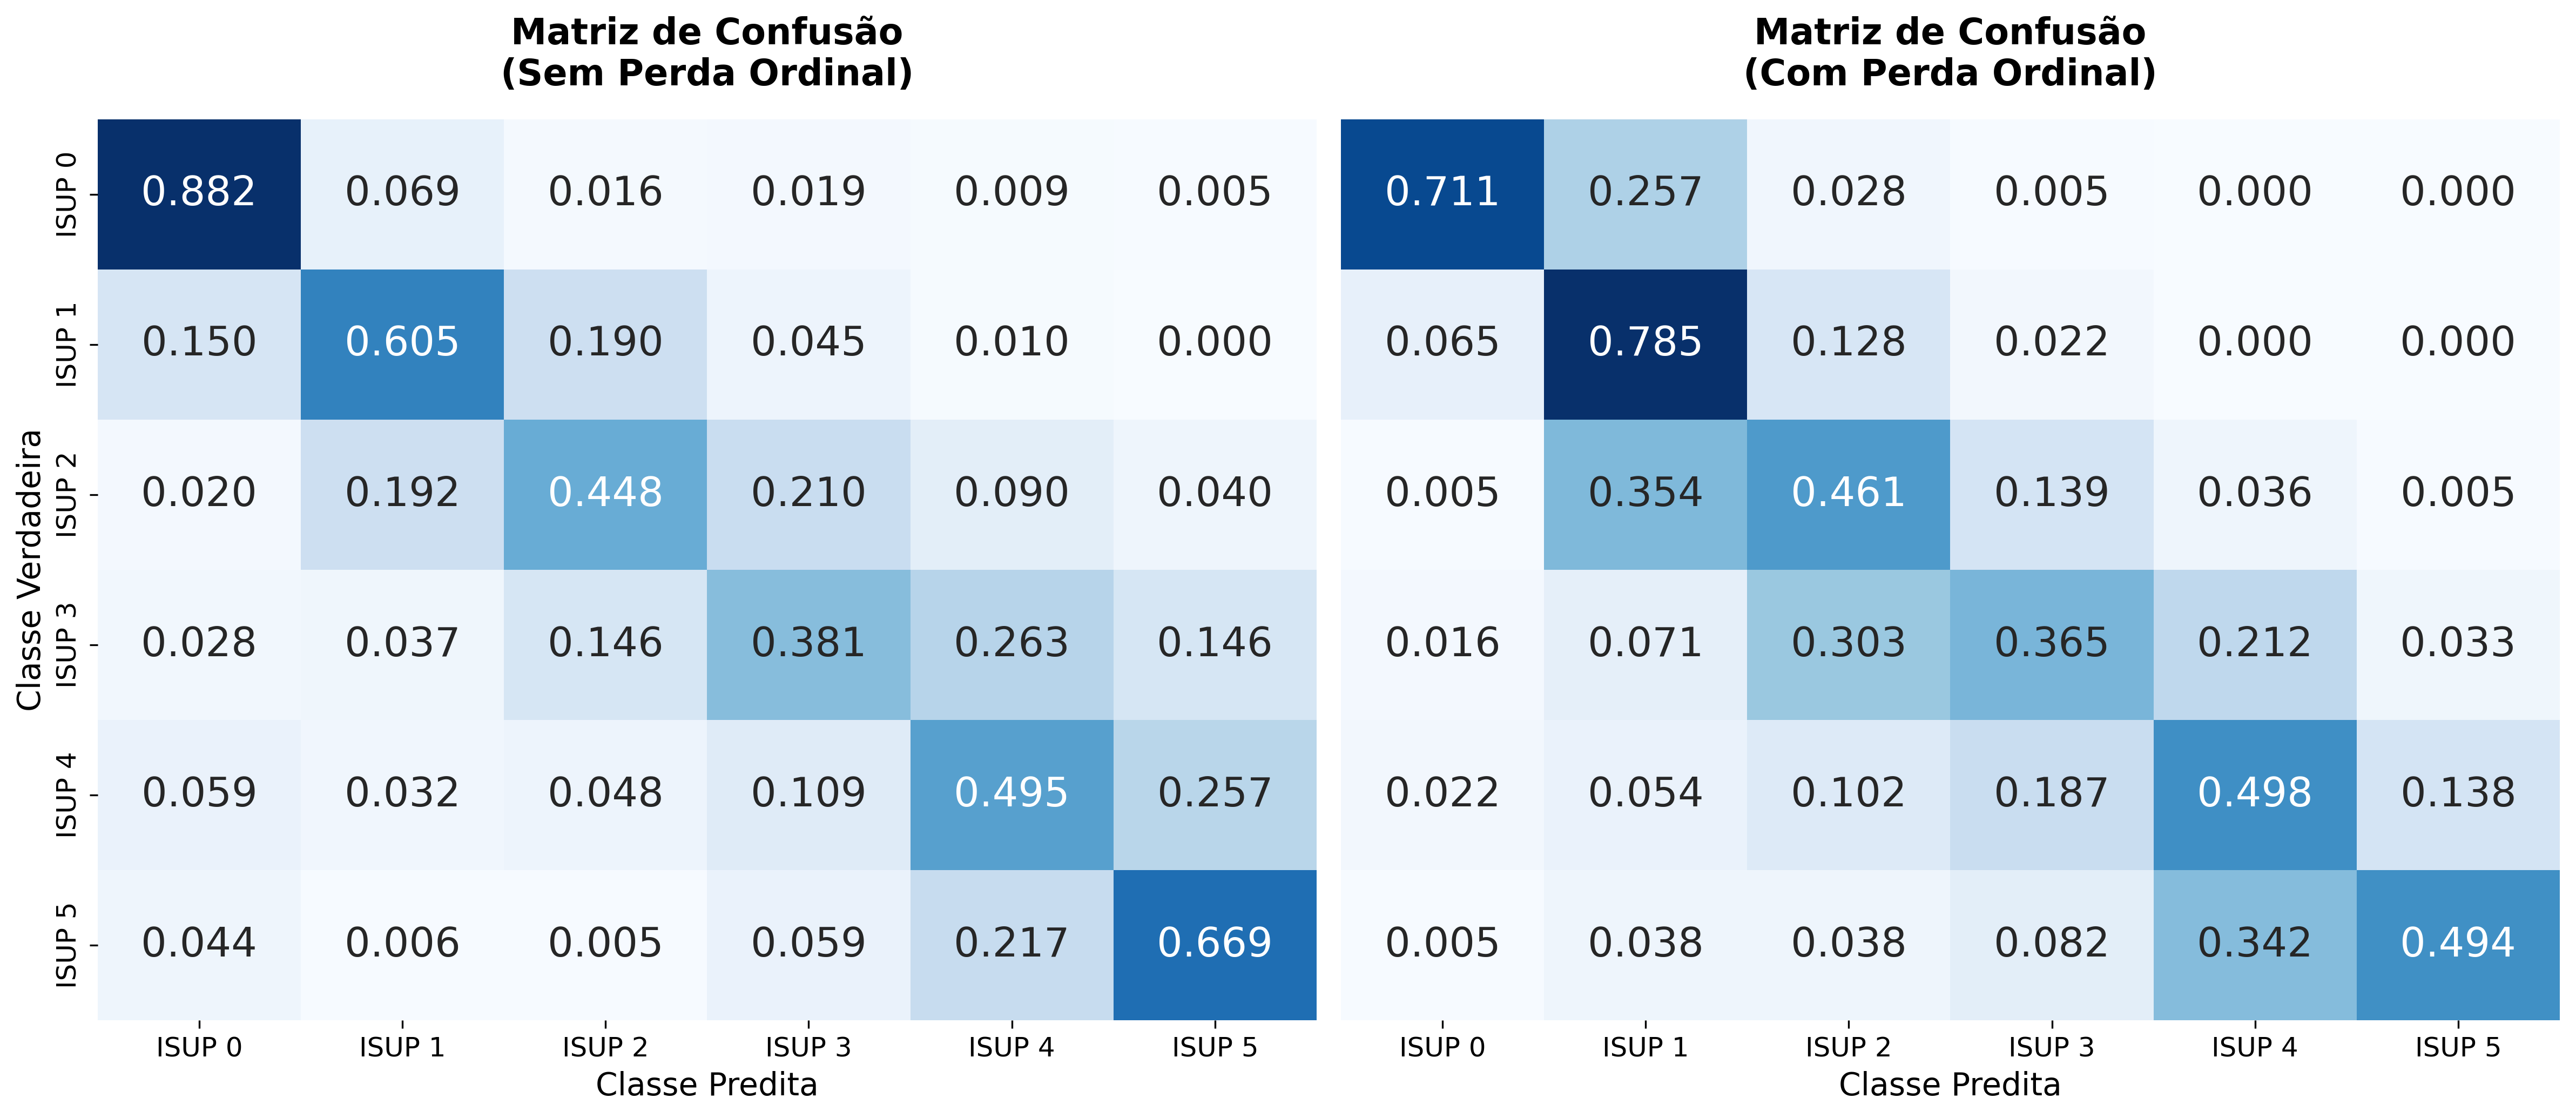
\includegraphics[width=1\linewidth]{figuras/confusion_matrices_baseline.png}
	\caption{Matrizes de confusão normalizadas obtidas para o modelo treinado com a função de perda BCE (à esquerda) e com a função de perda ordinal (à direita).}
	\label{fig:confusionmatricesbaseline}
\end{figure}

Ao analisar a diagonal principal das matrizes, observa-se melhora nas classes ISUP 1, ISUP 2 e ISUP 4, enquanto houve redução na acurácia das classes ISUP 0, ISUP 3 e ISUP 5. Além disso, a perda ordinal praticamente elimina erros entre classes distantes; amostras ISUP 0 deixam de ser classificadas como ISUP 3, 4 ou 5 e passam a apresentar confusão predominantemente com a classe adjacente ISUP 1. Em contrapartida, observa-se maior dispersão nas classes intermediárias, especialmente nas classes ISUP 2 e ISUP 3, o que reflete a dificuldade intrínseca de distinção entre graus histopatológicos adjacentes. Em síntese, os resultados indicam que a utilização da perda ordinal promove um comportamento de classificação mais alinhado à natureza hierárquica do problema, reduzindo discrepâncias severas entre classes e favorecendo confusões entre graus histopatológicos adjacentes.

Após a introdução da perda ordinal, observou-se que o desbalanceamento do conjunto de dados, descrito na Seção~\ref{sec:method_materiais}, poderia estar limitando o desempenho do modelo. Diante disso, foi proposta uma função de perda híbrida que combina penalização ordinal com o mecanismo focal, com o objetivo de enfatizar as amostras mais difíceis e mitigar os efeitos do desbalanceamento entre as classes.

Essa estratégia resultou no melhor desempenho entre as configurações avaliadas, atingindo $kappa = 0.856$ e acurácia de $0.669$. Em comparação com o modelo \textit{baseline}, essa abordagem proporcionou um ganho absoluto de aproximadamente $3\%$ em kappa e mais de 6 pontos percentuais em acurácia.

\begin{table}[!htb]
	\centering
	\resizebox{\textwidth}{!}{%
		\begin{tabular}{lcccccc}
			\toprule
			& \multicolumn{3}{c}{\textbf{Kappa Quadrático}} & \multicolumn{3}{c}{\textbf{Acurácia (\%)}} \\
			\cmidrule(lr){2-4} \cmidrule(lr){5-7}
			\textbf{Configuração} & \textbf{Resultado} & \textbf{Des. Pad.} & \textbf{IC 95\%} & \textbf{Resultado} & \textbf{Des. Pad.} & \textbf{IC 95\%} \\
			\midrule
			
			\quad BCE (baseline) 
			& 0.826 & 0.012 & [0.806; 0.846] 
			& 0.592 & 0.012 & [0.572; 0.612] \\
			
			\quad BCE + Remoção de Ruído 
			& 0.833 & 0.013 & [0.812; 0.853] 
			& 0.638 & 0.116 & [0.619; 0.657] \\
			
			\quad Perda Ordinal 
			& 0.851 & \textbf{0.009} & [0.833; 0.869] 
			& 0.608 & 0.126 & [0.587; 0.628] \\
			
			\quad \textbf{Ordinal + Focal (Híbrida)} 
			& \textbf{0.856} & 0.011 & [0.833; 0.876] 
			& \textbf{0.669} & 0.011 & [0.635; 0.683] \\
			
			\bottomrule
		\end{tabular}%
	}
	\caption{Impacto incremental das estratégias propostas no desempenho da EfficientNet-B0.}
	\label{tab:impacto_loss_expandido}
\end{table}

A análise das matrizes de confusão apresentadas na Figura~\ref{fig:cm_ordinal_focal} evidencia melhorias consistentes ao utilizar a perda focal ordinal. O modelo treinado apenas com perda ordinal apresenta maior dispersão nas classes intermediárias, particularmente na classe ISUP 3, cuja taxa de acerto foi de $0.365$, com uma parcela significativa das amostras confundida com ISUP 2 ($0.303$) e ISUP 4 ($0.212$). Em contraste, o modelo híbrido apresentou maior concentração das predições na diagonal principal, indicando maior capacidade discriminativa. Observam-se melhorias relevantes em diversas classes, incluindo ISUP 0 ($0.857$ vs.\ $0.711$), ISUP 3 ($0.492$ vs.\ $0.365$) e ISUP 4 ($0.652$ vs.\ $0.498$). Além disso, nota-se uma redução das confusões entre classes intermediárias, especialmente entre ISUP 2 e ISUP 3, o que sugere maior separabilidade entre esses graus histopatológicos.

Outro aspecto importante é a melhora na distinção entre classes de alto grau. No modelo ordinal, uma proporção significativa de amostras classificadas como ISUP 5 foi classificada como ISUP 4 ($0.342$). Embora essa confusão ainda esteja presente no modelo híbrido ($0.380$), observa-se um aumento na taxa de acerto para ISUP 4 ($0.652$ vs.\ $0.498$), indicando maior discriminação entre os graus superiores.

\begin{figure}[!htb]
	\centering
	\begin{subfigure}{0.47\textwidth}
		\centering
		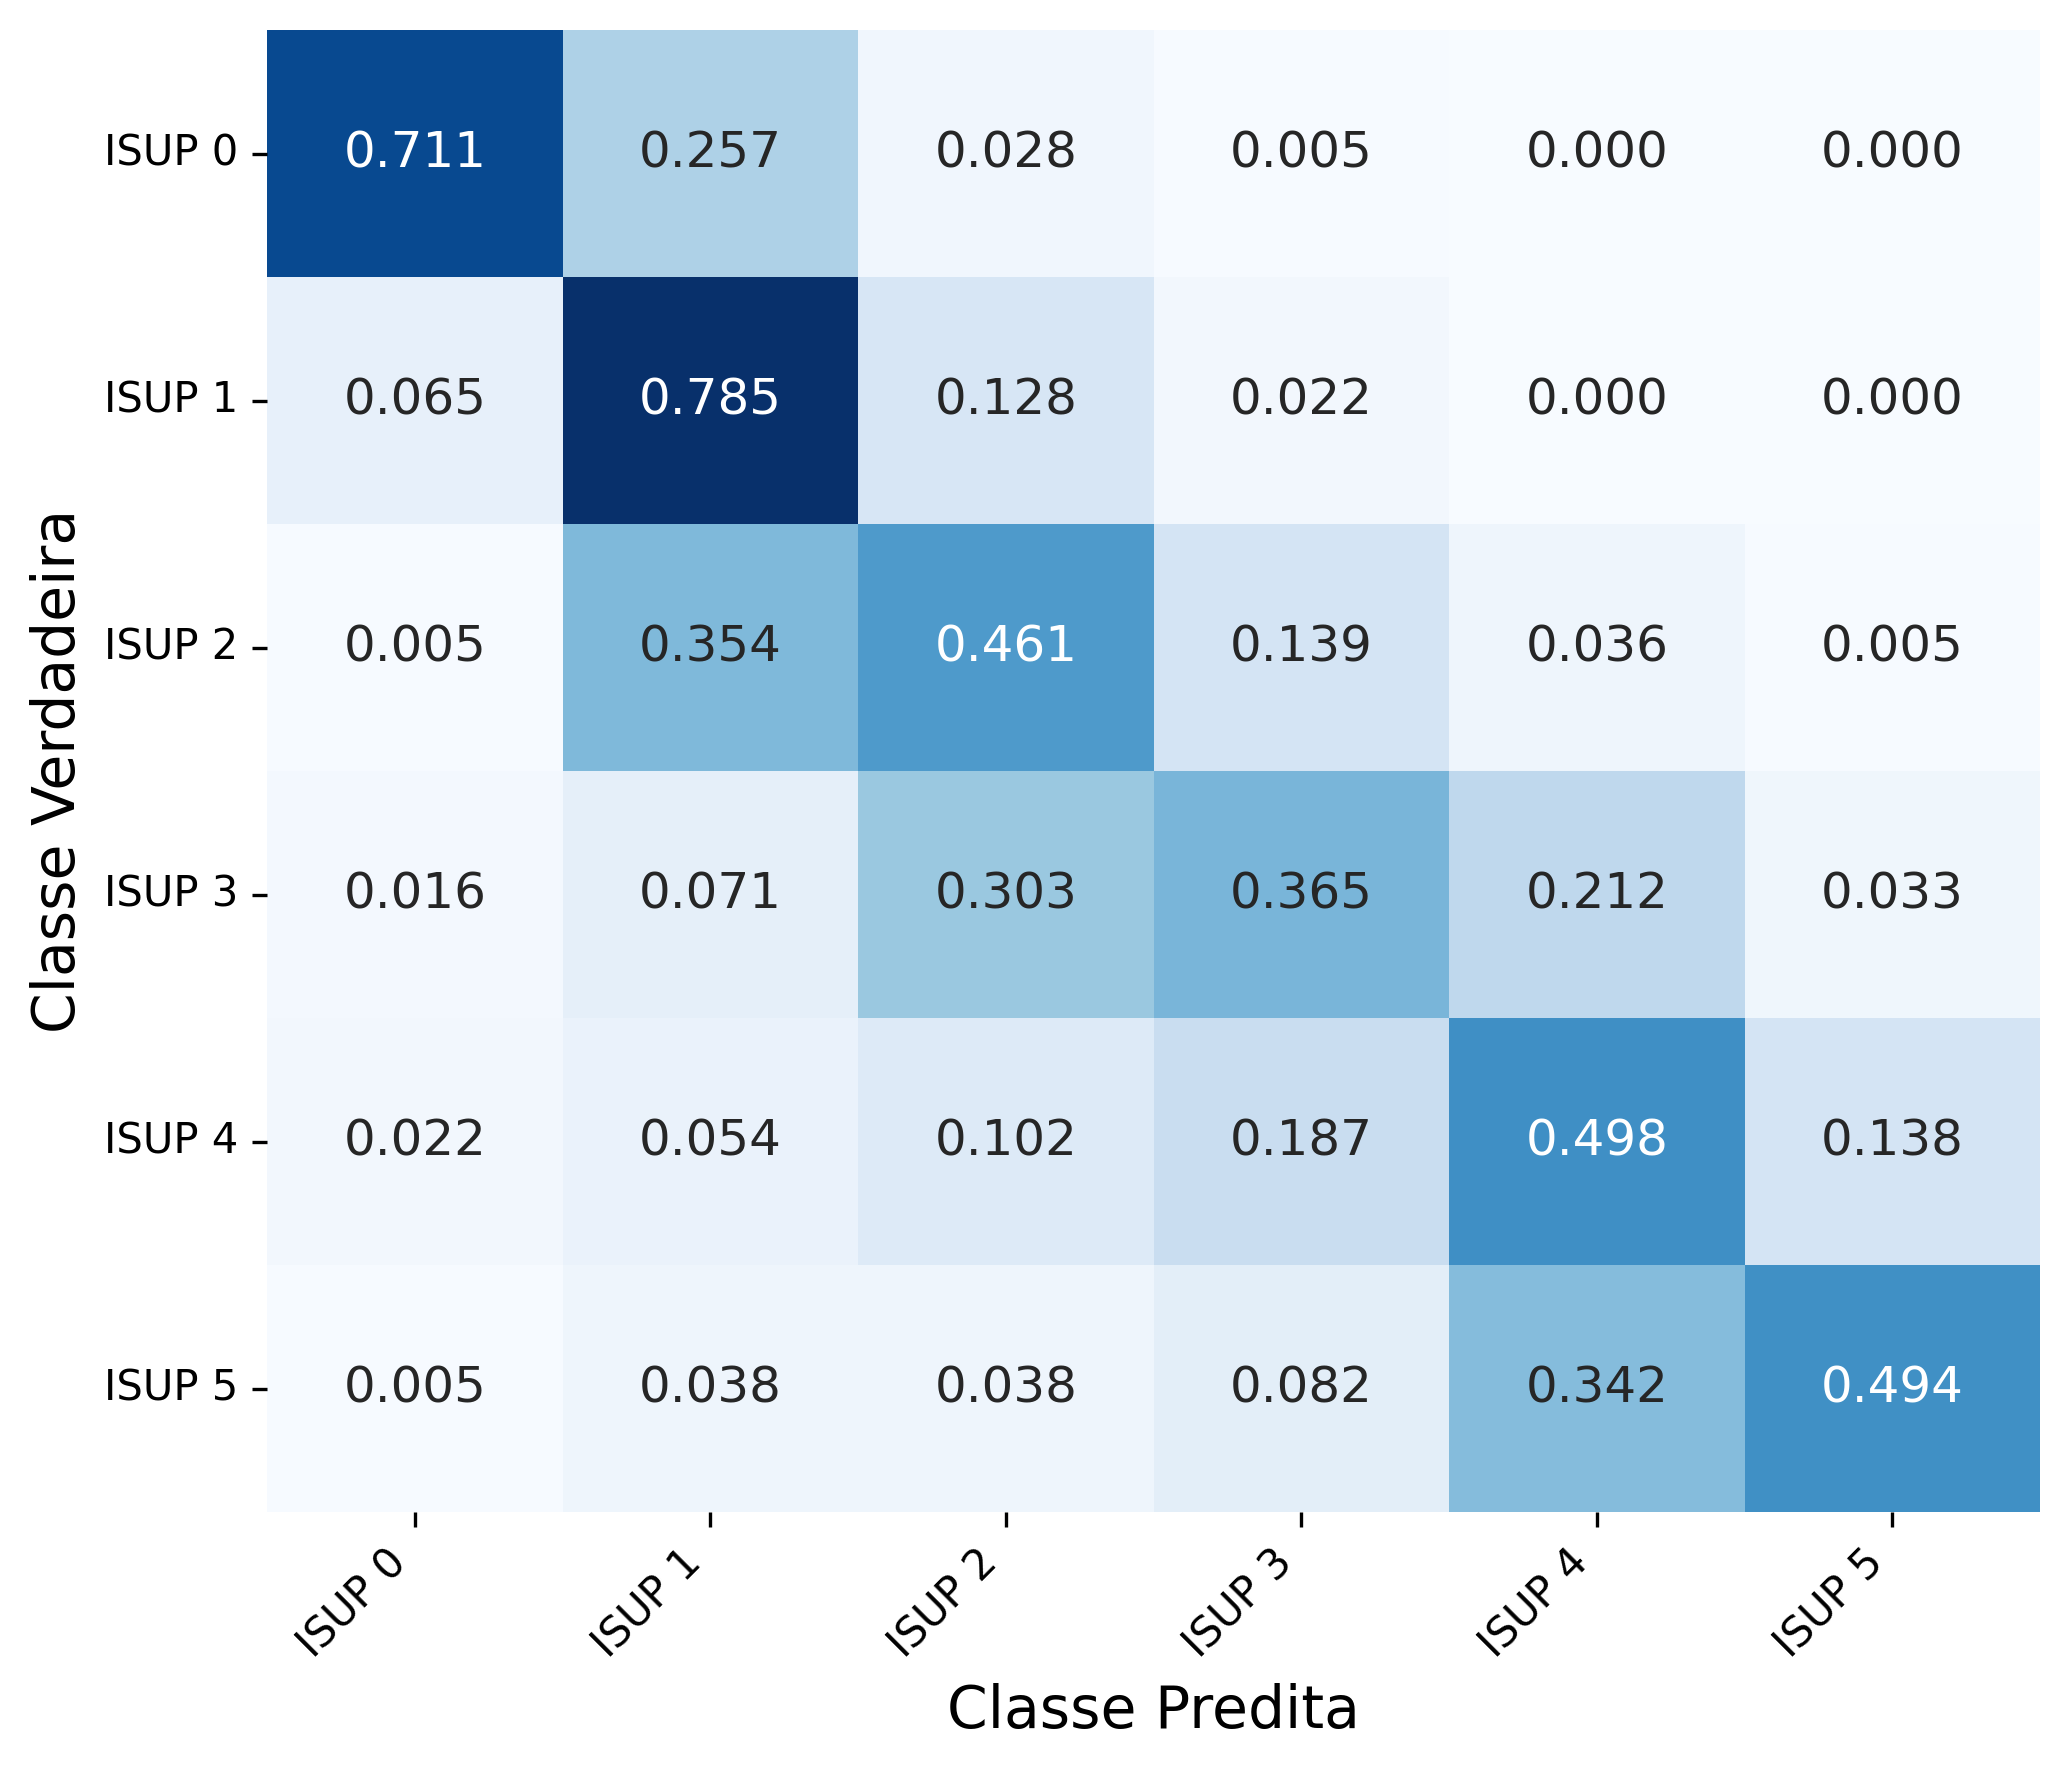
\includegraphics[width=\linewidth]{figuras/cm_ordinal.png}
		\caption{Ordinal}
		\label{subfig:ordinal}
	\end{subfigure}
	\hfill
	\begin{subfigure}{0.47\textwidth}
		\centering
		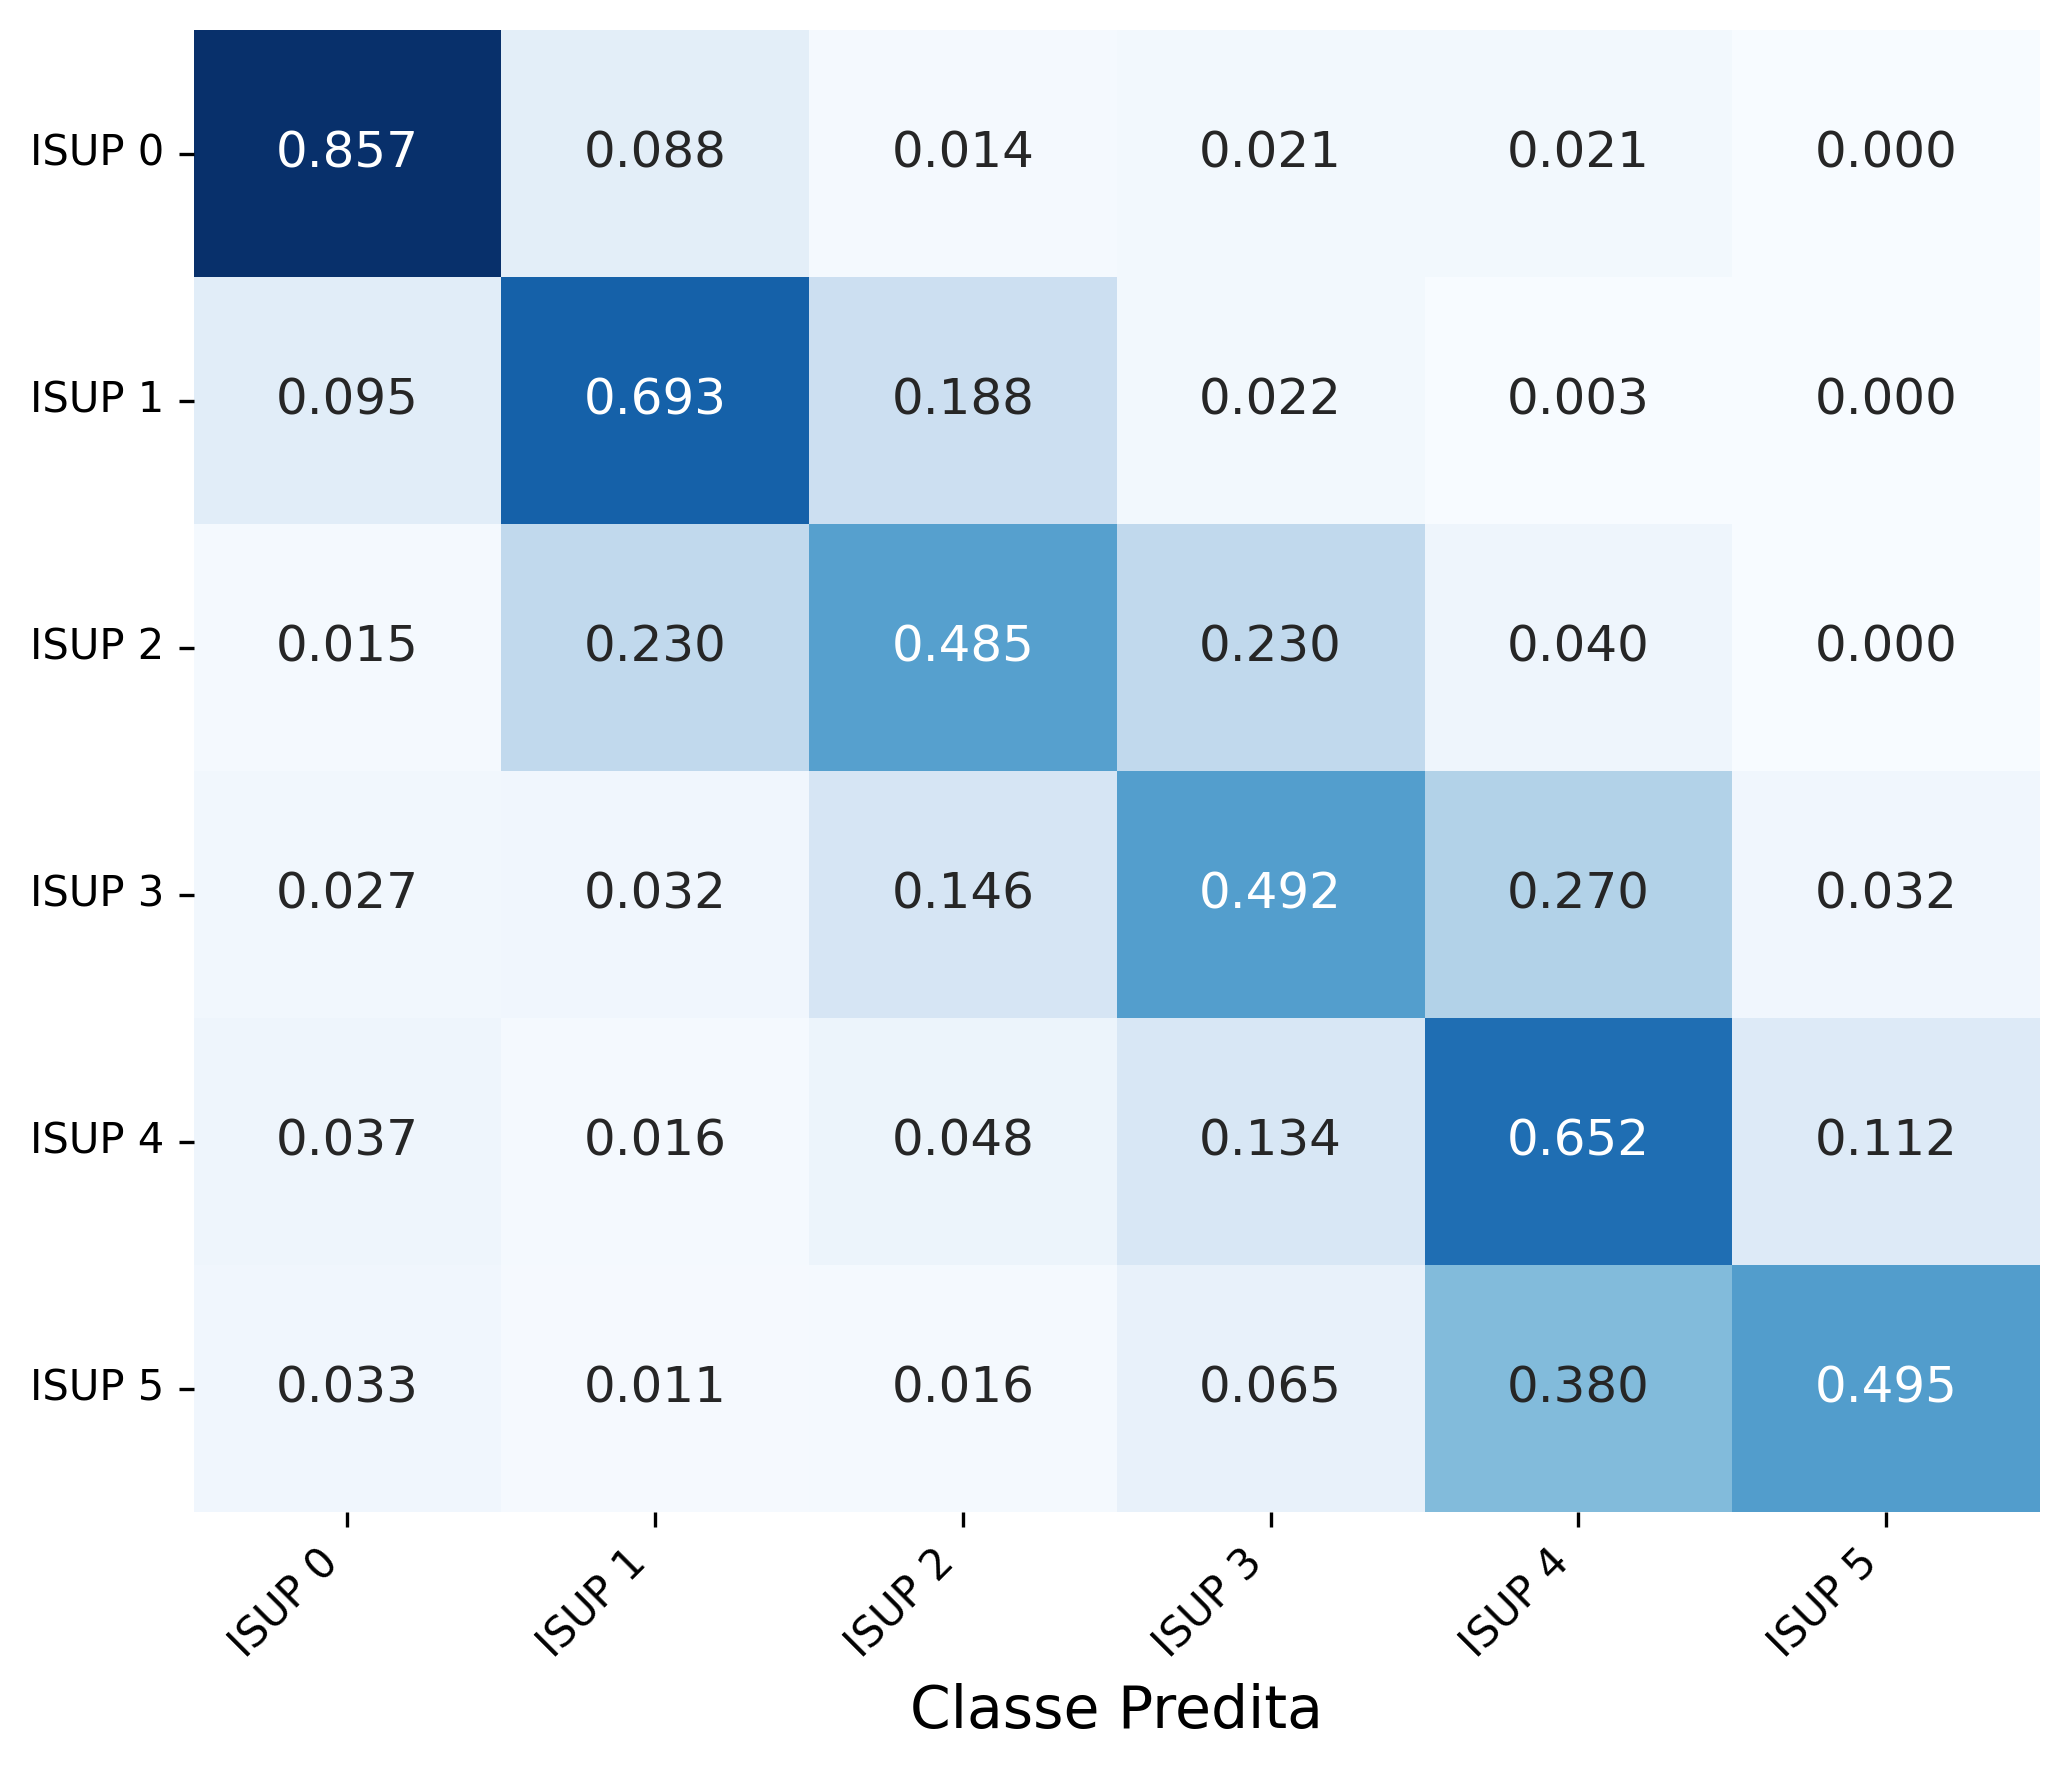
\includegraphics[width=\linewidth]{figuras/cm_ordinal_focal.png}
		\caption{Ordinal Focal}
		\label{subfig:ordinal_focal}
	\end{subfigure}
	\caption{Matrizes de confusão normalizadas para modelos treinados com perda ordinal e perda focal ordinal.}
	\label{fig:cm_ordinal_focal}
	
\end{figure}

\section{Comparação entre Arquiteturas EfficientNet}
\label{sec:comparable}
A configuração experimental definida para a EfficientNet-B0 também foi aplicada às arquiteturas EfficientNet-B3 e EfficientNet-B7, inclusive à função de perda híbrida. O objetivo foi avaliar se arquiteturas mais profundas poderiam gerar ganhos adicionais de desempenho.

Os resultados, apresentados na Tabela \ref{tab:comparacao_arquiteturas}, indicam que a EfficientNet-B0 apresentou o melhor desempenho tanto no kappa quadrático quanto na acurácia. As arquiteturas mais profundas não apresentaram melhorias significativas e, em alguns casos, exibiram uma leve redução nas métricas avaliadas.

Esse comportamento sugere que modelos mais complexos podem ser mais suscetíveis ao \textit{overfitting} neste conjunto de dados. Assim, a EfficientNet-B0 demonstrou o melhor equilíbrio entre desempenho preditivo, estabilidade estatística e custo computacional.

\begin{table}[!htb]
	\centering
	\resizebox{\textwidth}{!}{%
		\begin{tabular}{lcccccc}
			\toprule
			& \multicolumn{3}{c}{\textbf{Kappa Quadrático}} & \multicolumn{3}{c}{\textbf{Acurácia (\%)}} \\
			\cmidrule(lr){2-4} \cmidrule(lr){5-7}
			\textbf{Arquitetura} & \textbf{Resultado} & \textbf{Des. Pad.} & \textbf{IC 95\%} & \textbf{Resultado} & \textbf{Des. Pad.} & \textbf{IC 95\%} \\
			\midrule
			
			EfficientNet-B0 
			& \textbf{0.856} & 0.011 & [0.833; 0.876] 
			& \textbf{0.669} & 0.011 & [0.635; 0.683] \\
			
			EfficientNet-B3 
			& 0.849 & 0.013 & [0.824; 0.870] 
			& 0.661 & 0.014 & [0.634; 0.685] \\
			
			EfficientNet-B7 
			& 0.842 & 0.015 & [0.815; 0.866] 
			& 0.654 & 0.016 & [0.628; 0.678] \\
			
			\bottomrule
		\end{tabular}%
	}
	\caption{Comparação de desempenho entre as arquiteturas da família EfficientNet, utilizando a configuração experimental proposta.}
	\label{tab:comparacao_arquiteturas}
\end{table}

\section{Avaliação do \textit{Ensemble}}

Embora os modelos individuais apresentem desempenho competitivo, abordagens baseadas em \textit{ensemble} são amplamente utilizadas para melhorar a robustez e a capacidade de generalização de modelos de aprendizado profundo. A combinação de múltiplos classificadores permite reduzir a variância das predições e explorar complementaridades entre diferentes arquiteturas e estratégias de treinamento.

Com esse objetivo, foi construído um \textit{ensemble} composto pelos três modelos EfficientNet (B0, B3 e B7), descritos na Seção \ref{sec:comparable}. A combinação das predições foi investigada por meio de diferentes estratégias de agregação: média, máxima e votação majoritária. Os resultados obtidos são apresentados na Tabela~\ref{tab:ensemble_results}.

\begin{table}[!htb]
	\centering
	\resizebox{\textwidth}{!}{%
		\begin{tabular}{lcccccc}
			\toprule
			& \multicolumn{3}{c}{\textbf{Kappa Quadrático}} & \multicolumn{3}{c}{\textbf{Acurácia (\%)}} \\
			\cmidrule(lr){2-4} \cmidrule(lr){5-7}
			\textbf{Estratégia de Ensemble} & \textbf{Resultado} & \textbf{Des. Pad.} & \textbf{IC 95\%} & \textbf{Resultado} & \textbf{Des. Pad.} & \textbf{IC 95\%} \\
			\midrule
			
			Média 
			& \textbf{0.880} & 0.010 & [0.861; 0.898] 
			& \textbf{0.698} & 0.012 & [0.674; 0.721] \\
			
			Máxima 
			& 0.840 & 0.014 & [0.812; 0.864] 
			& 0.583 & 0.015 & [0.556; 0.610] \\
			
			Votação 
			& 0.860 & 0.012 & [0.835; 0.881] 
			& 0.692 & 0.013 & [0.667; 0.715] \\
			
			\bottomrule
		\end{tabular}%
	}
	\caption{Desempenho das diferentes estratégias de ensemble avaliadas no conjunto de teste.}
	\label{tab:ensemble_results}
\end{table}

Observa-se que as estratégias de ensemble baseadas em média e votação majoritária apresentaram desempenho superior ao dos modelos individuais, enquanto a estratégia baseada no operador máximo apresentou desempenho inferior. A estratégia de média simples obteve o melhor resultado global, com kappa de $0.880$ e acurácia de $0.698$. Em comparação com o melhor modelo individual (EfficientNet-B0 com perda ordinal focal), essa abordagem proporcionou um ganho absoluto de aproximadamente 2,3 pontos percentuais em kappa e de cerca de 3,8 pontos percentuais em acurácia.

Esse resultado sugere que as arquiteturas EfficientNet-B0, B3 e B7 capturam padrões complementares no conjunto de dados, permitindo que o \textit{ensemble} reduza erros individuais e produza predições mais estáveis. Em contraste, a estratégia baseada na seleção da probabilidade máxima apresentou desempenho inferior, indicando que a simples escolha da predição mais confiante não explora adequadamente a complementaridade entre os modelos. De forma geral, os resultados demonstram que o uso de \textit{ensemble} contribui para melhorar a capacidade preditiva do sistema, fornecendo estimativas mais robustas e reduzindo a variabilidade associada às decisões de modelos individuais.

\section{Comparação com trabalhos relacionados}

Nesta seção, apresenta-se uma análise comparativa entre o método proposto e os trabalhos relacionados discutidos no Capítulo \ref{cap:trabalhos-relacionados}. A Tabela \ref{tab:comparacao_estado_arte} sintetiza essas abordagens, reunindo informações sobre o \textit{dataset} utilizado, o modelo principal, o nível de análise (em nível de \textit{patch} ou WSI), a tarefa considerada (incluindo número de classes e tipo de graduação, como Gleason ou ISUP), bem como as métricas de desempenho reportadas, especificamente acurácia e coeficiente kappa.

\begin{table}[htb]
	\centering
	\scriptsize
	\setlength{\tabcolsep}{3pt}
	\renewcommand{\arraystretch}{1.0}
	
	\resizebox{\linewidth}{!}{
		\begin{tabular}{llllccc}
			\toprule
			\textbf{Trab.} & \textbf{Dados} & \textbf{Modelo} & \textbf{Nível} & \textbf{Tarefa} & \textbf{Acc.} & \textbf{kappa} \\
			\midrule
			
			\cite{pyramidalcnn} 
			& Radboud 
			& Pyramidal CNN 
			& Patch $\rightarrow$ WSI 
			& Gleason / GG 
			& 0,773 
			& - \\
			
			\cite{ikromjanov2021vit_prostate} 
			& PANDA 
			& ViT 
			& Patch
			& Gleason 
			& 0,800 
			& - \\
			
			\cite{Xiang2023Prostate} 
			& PANDA 
			& ResNet50 + GCN 
			& WSI
			& ISUP 
			& - 
			& 0,931 / 0,801 \\
			
			\cite{alici2024efficient}
			& DiagSet 
			& EffNet-B4 + ECA 
			& Patch
			& Bin./4 cls 
			& 0,961 / 0,948 
			& - \\
			
			\cite{kosoko2024xai_prostate}
			& SICAPv2 
			& VGG19 
			& Patch
			& Gleason 
			& 0,780 
			& - \\			
			
			\cite{bhattacharyya2024wsi}
			& PANDA
			& EffNet-B1 + MIL + Ensemble
			& WSI
			& ISUP
			& -
			& 0,881 \\ 
			
			\cite{kabir2025automating}
			& PANDA
			& EffNet-B0 + DeepLabV3 + RF
			& WSI + Seg
			& ISUP
			& -
			& 0,921 \\
			
			\cite{bhattacharyya2026tsor}
			& PANDA / SICAPv2
			& SSL (TSOR) + Ord. Reg.
			& WSI
			& ISUP
			& -
			& 0,884 \\ 
			
			\midrule
			
			\textbf{Proposto (Base)} 
			& \textbf{PANDA} 
			& \textbf{EffNet-B0 + Ord. Focal} 
			& \textbf{WSI}
			& \textbf{ISUP} 
			& \textbf{0,669} 
			& \textbf{0,856} \\
			
			\textbf{Proposto (Ensemble)} 
			& \textbf{PANDA} 
			& \textbf{EffNet-B0/B3/B7 + Ensemble} 
			& \textbf{WSI}
			& \textbf{ISUP} 
			& \textbf{0,698} 
			& \textbf{0,880} \\
			
			\bottomrule
		\end{tabular}
	}
	
	\caption{Comparação do método proposto com trabalhos recentes.}
	\label{tab:comparacao_estado_arte}
\end{table}

Embora diferentes trabalhos reportem resultados competitivos na classificação do padrão de Gleason, diversas limitações metodológicas reduzem sua aplicabilidade clínica e comprometem a generalização dos modelos.

No caso de \cite{pyramidalcnn}, a abordagem baseada em uma arquitetura piramidal acarreta alto custo computacional, exigindo o treinamento de múltiplas CNNs e o processamento de mais de 10 milhões de \textit{patches}. Além disso, o uso de subamostragem severa para o balanceamento resulta no descarte de um grande volume de informação clínica relevante. De forma semelhante, \cite{ikromjanov2021vit_prostate}, \cite{alici2024efficient} e \cite{kosoko2024xai_prostate} restringem a tarefa à classificação de \textit{patches}, o que simplifica o problema e dificulta comparações diretas com abordagens em nível de WSI. No caso específico de \cite{ikromjanov2021vit_prostate}, há ainda a exclusão da coorte do \textit{Karolinska} e dependência de máscaras de segmentação, reduzindo a variabilidade dos dados e favorecendo resultados potencialmente superestimados.

Outros trabalhos também apresentam fragilidades relacionadas à curadoria de dados e à robustez. \cite{Xiang2023Prostate} reporta um \textit{kappa} alto (0,931), porém obtido em um conjunto interno sem artefatos reais (como marcas de caneta), com queda significativa na validação externa (0,801), o que evidencia limitações de generalização. De forma análoga, \cite{kabir2025automating} depende de anotações em nível de pixel, o que restringe drasticamente o volume de dados utilizado e cria um cenário pouco representativo da prática clínica. Limitações semelhantes na amostragem são observadas em \cite{bhattacharyya2026tsor} e \cite{bhattacharyya2024wsi}, que utilizam apenas frações do dataset PANDA. Especificamente em \cite{bhattacharyya2024wsi}, embora o método baseado em \textit{ensemble} reporte um \textit{kappa} competitivo de 0,881, os autores aplicam um balanceamento manual forçado em todo o conjunto de dados, selecionando o mesmo número de imagens para cada grau ISUP, antes mesmo de separar os conjuntos de validação e teste. Essa abordagem mascara a distribuição real e severamente desbalanceada da doença na prática clínica, o que introduz um viés de avaliação e compromete a generalização do modelo para cenários do mundo real.

Em contraste, o método proposto elimina a dependência de anotações em nível de pixel por meio de uma filtragem automatizada baseada na entropia, permitindo o uso mais amplo e realista dos dados disponíveis. A abordagem opera diretamente no nível de WSI, evitando simplificações inerentes à análise por \textit{patches} e preservando a distribuição original das classes, sem descartar amostras arbitrariamente. Adicionalmente, o uso de regressão ordinal incorpora a estrutura hierárquica dos graus de Gleason, o que resulta em predições mais consistentes do ponto de vista clínico. Em conjunto, essas características conferem maior robustez, eficiência computacional e capacidade de generalização ao método proposto.

\section{Discussão}
\begin{comment}
	Os resultados obtidos evidenciam que a avaliação de modelos de classificação de câncer de próstata não deve se restringir à acurácia global, especialmente em problemas de estrutura ordinal e de impacto clínico direto. Abordagens que simplificam a tarefa, como classificações binárias ou nominais, tendem a apresentar melhor desempenho em métricas tradicionais, porém não modelam explicitamente a relação ordinal entre as classes, o que limita a interpretação clínica das predições.
	
	O método proposto se diferencia ao incorporar explicitamente a natureza ordinal dos graus ISUP, o que resulta em um aumento consistente do coeficiente kappa quadrático. Essa métrica é mais adequada ao problema, pois penaliza de forma mais severa erros entre classes distantes, refletindo melhor o impacto clínico das predições. A utilização da perda ordinal, especialmente quando combinada ao mecanismo de \textit{focal loss}, altera o padrão de erros do modelo. Observa-se maior concentração de confusões entre classes adjacentes, o que indica que o modelo captura a progressão gradual da doença, em vez de tratá-las como categorias independentes.
	
	O uso de estratégias de \textit{ensemble} mostrou-se fundamental para a melhoria do desempenho. A combinação de múltiplos modelos reduziu a variância das predições e aumentou a estabilidade dos resultados, resultando em ganhos adicionais no coeficiente \textit{kappa} e maior confiabilidade nas decisões. Esse efeito é particularmente relevante em cenários médicos. Adicionalmente, a filtragem de amostras com base na entropia contribuiu para a remoção de instâncias ruidosas ou ambíguas, melhorando a capacidade de generalização do modelo. Esse resultado evidencia a importância da qualidade dos dados em aplicações de aprendizado profundo, especialmente em contextos com variabilidade interobservador.
	
	A combinação das estratégias propostas, modelagem ordinal, \textit{focal loss}, \textit{ensemble} e filtragem por entropia, resultou em ganhos progressivos de desempenho, culminando em um modelo mais robusto e clinicamente coerente. Embora a acurácia global seja inferior à de alguns trabalhos da literatura, o método apresenta melhor alinhamento com a natureza ordinal do problema e maior relevância prática.
	
	Como limitação, destaca-se a utilização de um único conjunto de dados, o que pode comprometer a generalização dos resultados. Trabalhos futuros devem considerar validações externas, bem como a exploração de técnicas adicionais, como otimização bayesiana de hiperparâmetros e métodos mais avançados de \textit{ensemble}, visando aprimorar ainda mais a robustez e o desempenho do modelo.
\end{comment}

Os resultados obtidos evidenciam que a avaliação de modelos de classificação de câncer de próstata não deve se restringir à acurácia global, especialmente em problemas de estrutura ordinal e de impacto clínico direto. Abordagens que simplificam a tarefa, como classificações binárias ou nominais, tendem a apresentar melhor desempenho em métricas tradicionais, porém não modelam explicitamente a relação ordinal entre as classes, o que limita a interpretação clínica das predições.

O método proposto se diferencia ao incorporar explicitamente a natureza ordinal dos graus ISUP, o que resulta em um aumento consistente do coeficiente kappa quadrático. Essa métrica é mais adequada ao problema, pois penaliza de forma mais severa erros entre classes distantes, refletindo melhor o impacto clínico das predições. A utilização da perda ordinal, especialmente quando combinada ao mecanismo de \textit{focal loss}, altera o padrão de erros do modelo. Observa-se maior concentração de confusões entre classes adjacentes, o que indica que o modelo captura a progressão gradual da doença, em vez de tratá-las como categorias independentes.

O uso de estratégias de \textit{ensemble} mostrou-se fundamental não apenas para aumentar a estabilidade do modelo, mas também para recuperar casos de alta complexidade diagnóstica. A análise evidenciou que, em 70 instâncias, apenas um dos modelos individuais foi capaz de realizar a classificação correta — sendo 30 acertos do $\text{B0}$, 25 do $\text{B3}$ e 15 do $\text{B7}$. Nessas situações, o \textit{ensemble} foi capaz de consolidar corretamente o diagnóstico ao integrar as diferentes previsões, mesmo quando a maioria dos modelos falhava. Esse resultado é clinicamente relevante, pois demonstra que a diversidade arquitetural funciona como uma espécie de mecanismo de compensação: erros específicos de um modelo são corrigidos pelos acertos de outro. Na prática, isso implica que, caso apenas um único modelo fosse utilizado, essas 70 amostras apresentariam um alto risco de classificação incorreta, com uma taxa de erro potencial de pelo menos 57\%. Assim, o \textit{ensemble} não apenas melhora o desempenho médio, mas atua diretamente na redução de erros críticos, especialmente em casos mais desafiadores.

Além disso, observou-se um efeito complementar em 9 casos, nos quais todos os modelos individuais falharam isoladamente, mas a agregação por meio do \textit{ensemble mean} resultou na classificação correta. Esse achado indica que a combinação das probabilidades permite que a classe correta seja identificada a partir da distribuição conjunta das previsões, mesmo quando ela não apresenta a maior probabilidade em nenhum modelo individual. Por fim, a robustez da abordagem é reforçada pelo fato de que o \textit{ensemble} não introduziu erros em situações em que houve consenso correto entre os três modelos, preservando o desempenho nos casos já bem resolvidos.

A filtragem de amostras com base na entropia também contribuiu para a remoção de instâncias ruidosas ou ambíguas, melhorando a capacidade de generalização. Esse resultado evidencia a importância da qualidade dos dados em aplicações de aprendizado profundo, especialmente em contextos com alta variabilidade interobservador. A combinação das estratégias propostas, modelagem ordinal, \textit{focal loss}, \textit{ensemble} e filtragem por entropia, resultou em ganhos progressivos de desempenho, culminando em um sistema mais robusto e clinicamente coerente.

Como limitação, destaca-se a utilização de um único conjunto de dados, o que pode comprometer a generalização dos resultados. Trabalhos futuros devem considerar validações externas, bem como a exploração de técnicas adicionais, como otimização bayesiana de hiperparâmetros e métodos mais avançados de fusão de modelos, visando aprimorar ainda mais a robustez e o desempenho do sistema em biópsias fragmentadas.
\section{Estudo de Caso 1 - Erro clinicamente grave}
A análise dos resultados do ensemble revelou que 271 instâncias (17\%) do conjunto de teste não foram corretamente classificadas por nenhum dos modelos avaliados. Dentre elas, há casos clinicamente críticos. Por exemplo, o primeiro estudo de caso refere-se a uma WSI rotulada como ISUP 5, que foi consistentemente classificada como ISUP 0 por todos os três modelos e pelas estratégias de \textit{ensemble}.

\begin{figure}[H]
	\centering
	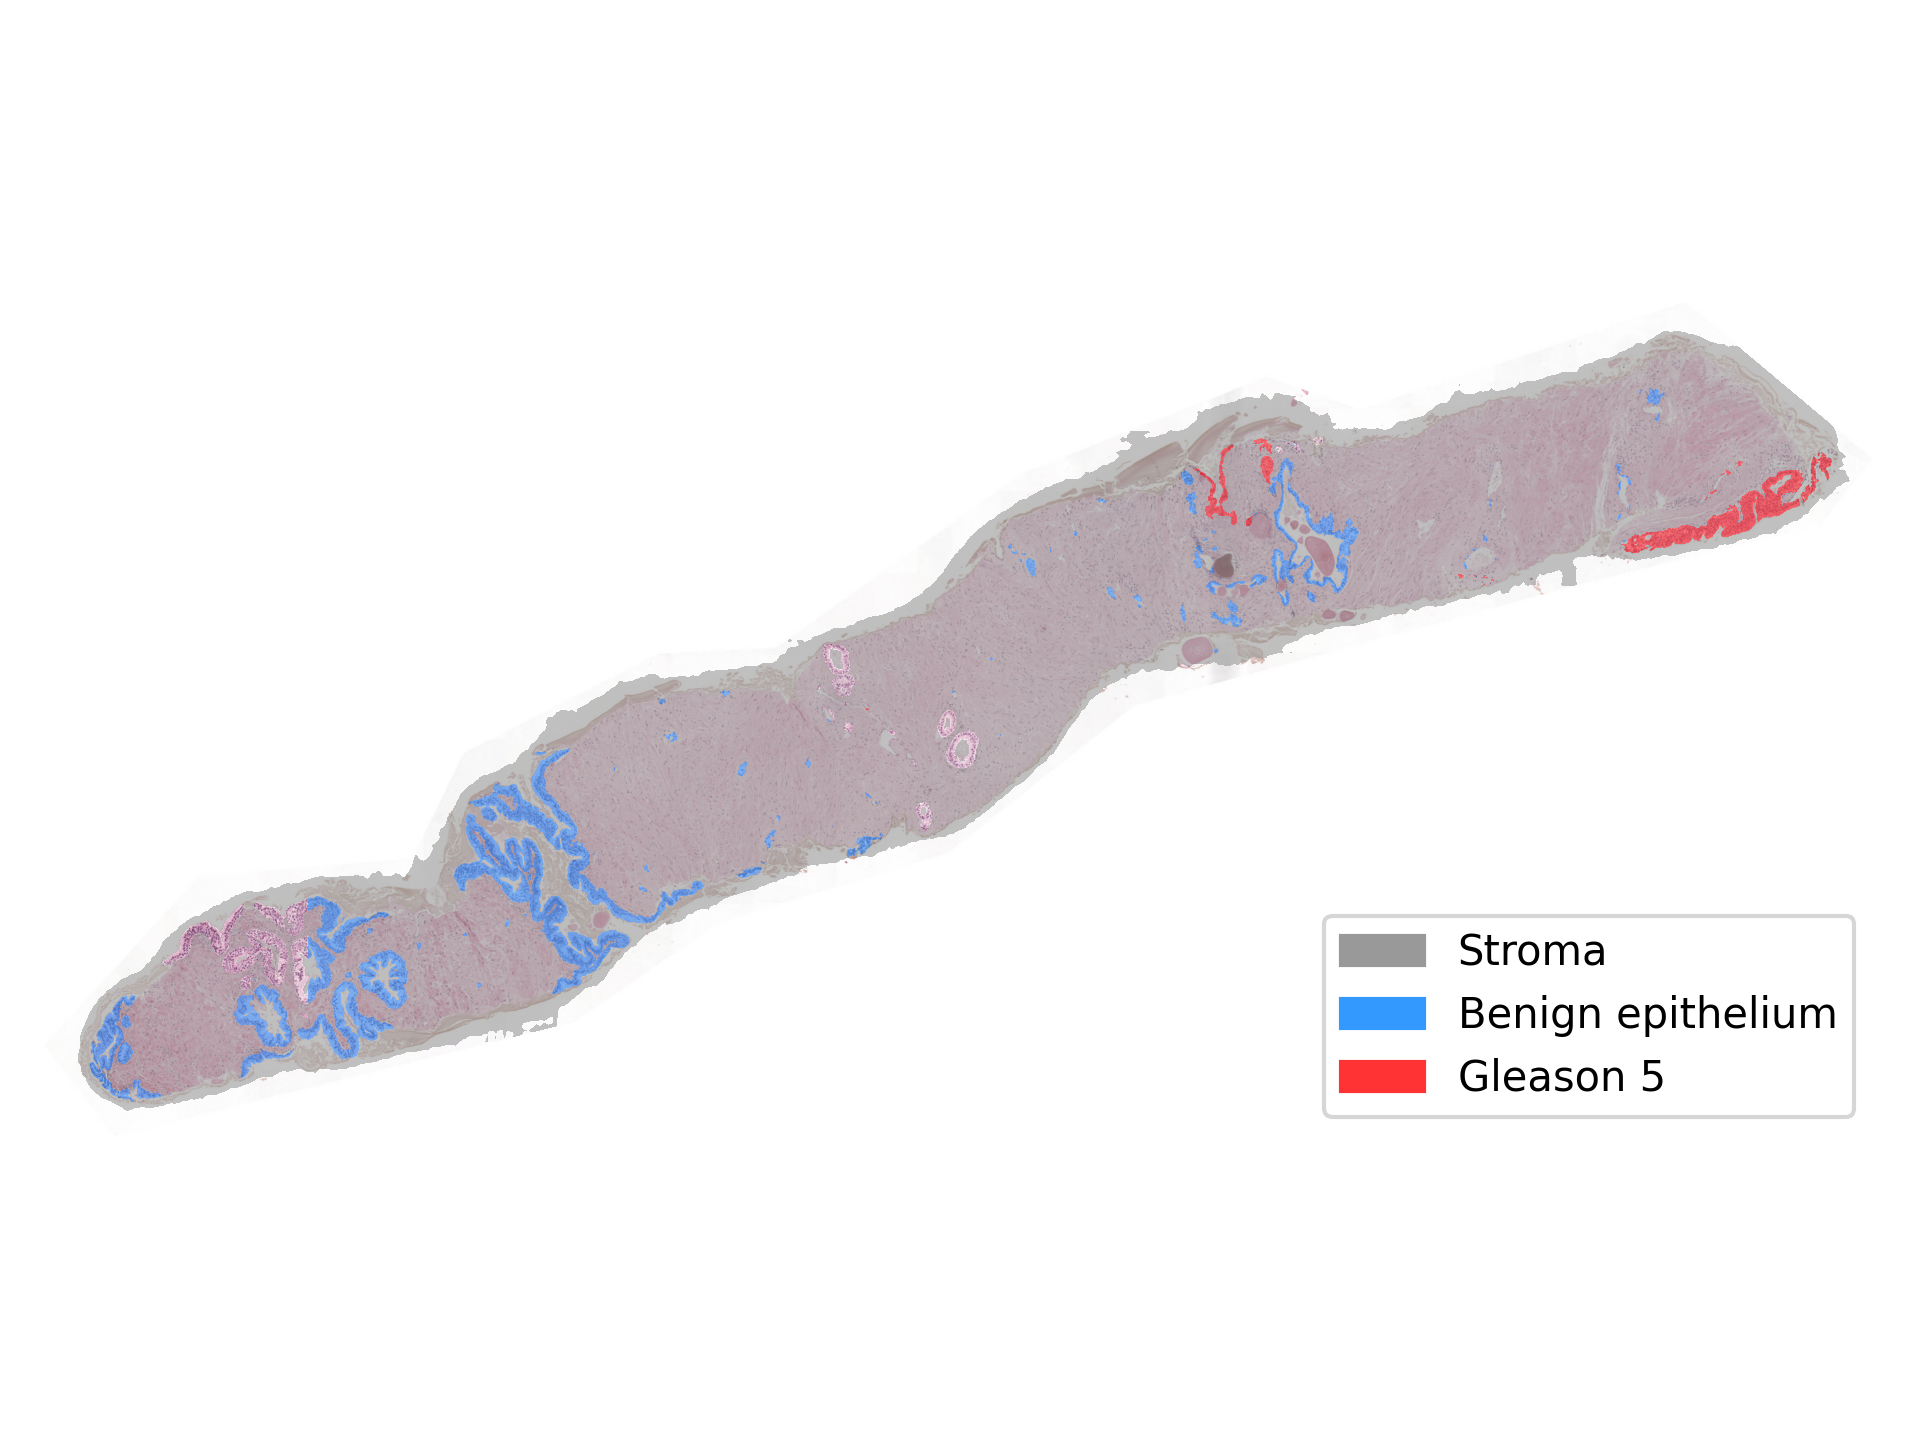
\includegraphics[width=0.8\linewidth]{figuras/mask}
	\caption{Exemplo de WSI classificada incorretamente.}
	\label{fig:mask}
\end{figure}

A Figura~\ref{fig:mask} evidencia a causa da classificação incorreta. Observa-se que grande parte do tecido corresponde a regiões benignas, enquanto apenas uma porção menor apresenta padrão de Gleason 5. Esse desbalanceamento pode levar os modelos a aprender representações dominadas por tecido benigno, enviesando a predição para classes de menor grau.

Entretanto, do ponto de vista clínico, o sistema de graduação ISUP considera exclusivamente as regiões cancerígenas na definição do grupo final, desconsiderando o tecido benigno. Assim, apesar da predominância de áreas benignas, a classificação correta dessa WSI é ISUP 5, devido à presença de regiões tumorais de alto grau. Essa discrepância evidencia uma limitação das abordagens baseadas em \textit{patches}, nas quais a contribuição das diferentes regiões não reflete sua relevância clínica, podendo levar à subvalorização de padrões mais agressivos.

\section{Estudo de Caso 2 - Erro adjacente}

Em contraste com o erro grave discutido anteriormente, este estudo de caso aborda um erro adjacente, no qual os modelos identificam corretamente a presença de malignidade e o padrão predominante, mas falham em capturar o padrão secundário de maior agressividade. Neste cenário, analisamos uma WSI com rótulo ISUP 5 (Gleason 4+5=9), que foi consistentemente classificada pelo como ISUP 4 (Gleason 4+4=8), tanto pelos modelos individuais quanto pelas estratégias de \textit{ensemble}.

\begin{figure}[H]
	\centering
	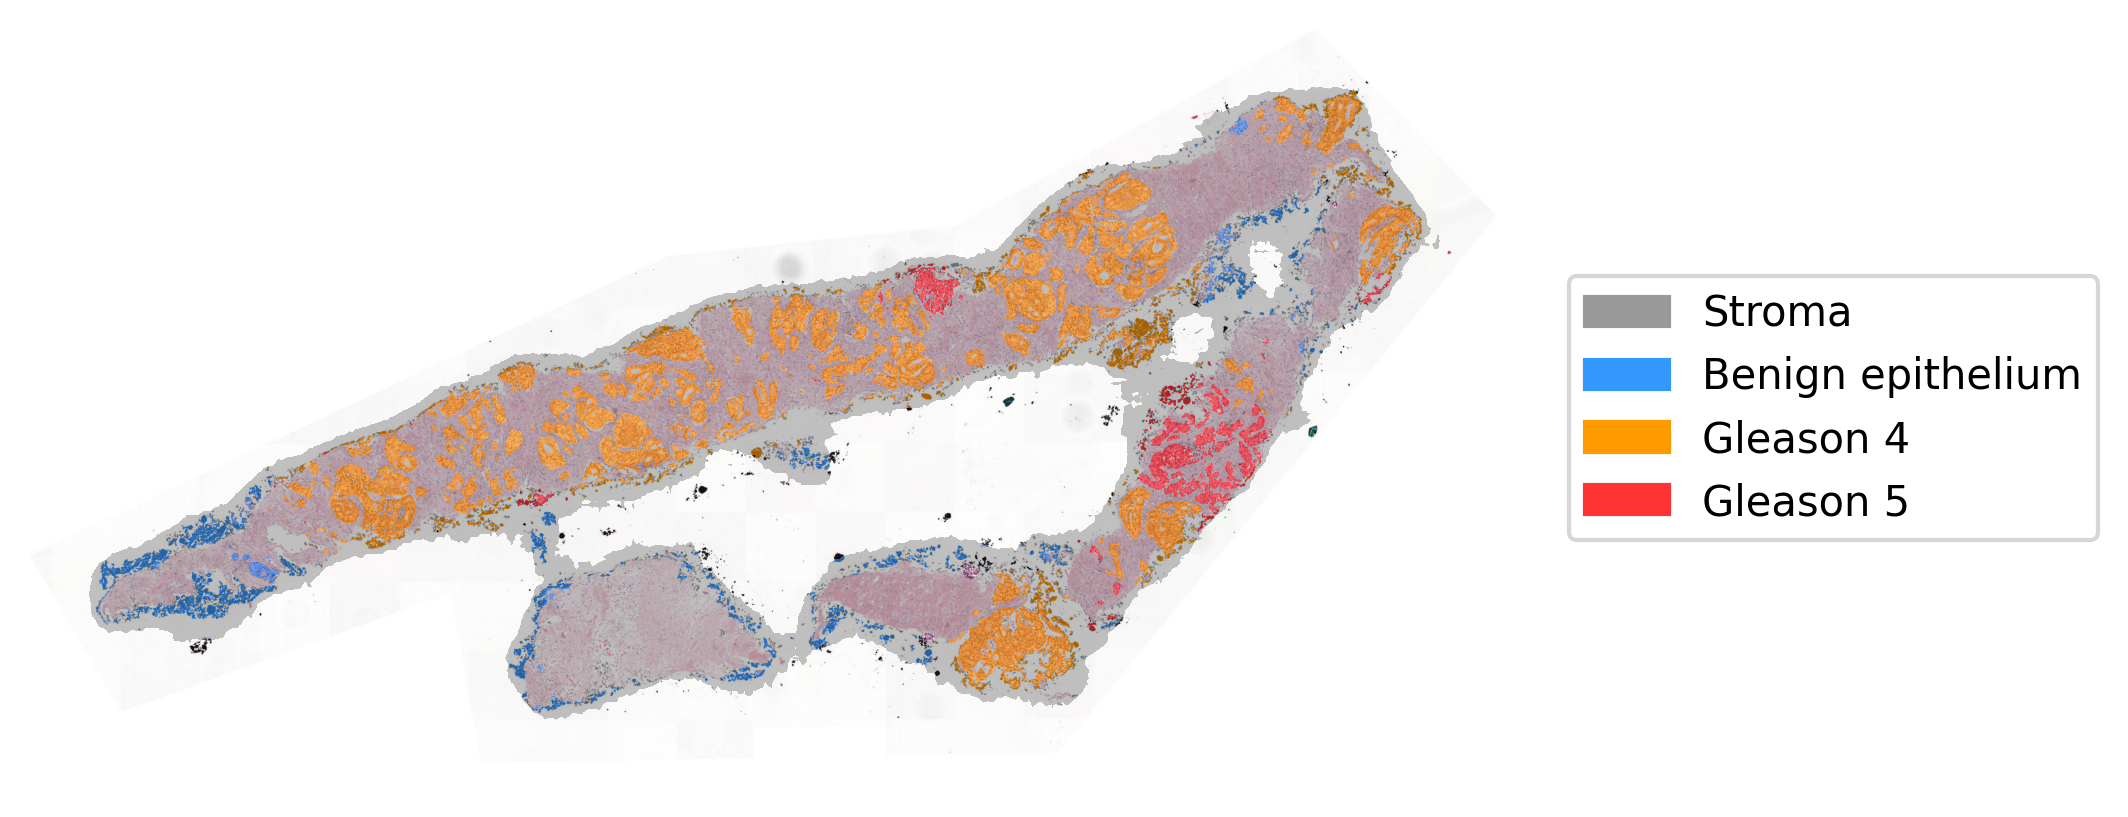
\includegraphics[width=0.8\linewidth]{figuras/mask_adjascente}
	\caption{Exemplo de WSI com erro adjacente (ISUP 5 classificada como ISUP 4).}
	\label{fig:mask_adjacente}
\end{figure}

A Figura~\ref{fig:mask_adjacente} mostra a predominância de tecido tumoral na amostra, majoritariamente composto pelo padrão de Gleason 4. Entretanto, há focos minoritários de padrão 5, que são determinantes para a classificação correta como ISUP 5. Do ponto de vista computacional, a predominância de \textit{patches} representando o padrão 4 reduz o impacto dos poucos \textit{patches} com padrão 5 na representação final, levando ao subestadiamento. Esse comportamento evidencia a dificuldade dos modelos em capturar padrões raros, mas clinicamente decisivos, especialmente quando há forte desbalanceamento entre os padrões e diferenças morfológicas sutis entre eles.

\section{Estudo de Caso 3 - Concordância unânime em lesão homogênea}

Diferentemente dos casos anteriores, este exemplo apresenta um cenário de alta concordância, no qual todos os modelos individuais e estratégias de \textit{ensemble} classificaram corretamente a WSI como ISUP 1.

\begin{figure}[H]
	\centering
	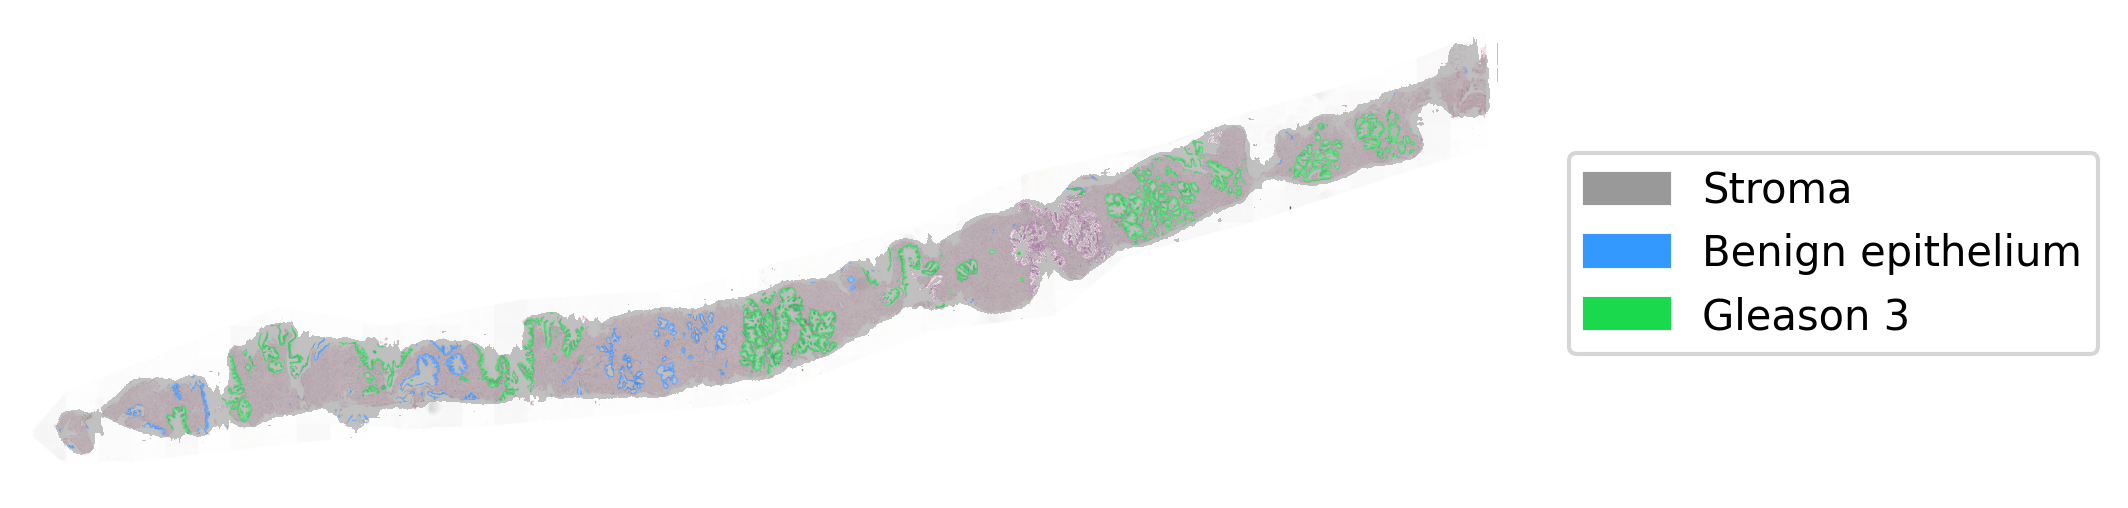
\includegraphics[width=0.8\linewidth]{figuras/6f0935638b47295c4e35008366c8768b}
	\caption{Exemplo de WSI com predição correta e unânime pelo \textit{ensemble}.}
	\label{fig:mask_concordance}
\end{figure}

A Figura~\ref{fig:mask_concordance} evidencia uma extensa e homogênea área tumoral composta predominantemente pelo padrão de Gleason 3. A ausência de padrões concorrentes e a ampla representatividade desse padrão favorecem a extração de características consistentes.

Do ponto de vista computacional, a predominância de \textit{patches} representativos da classe correta reduz ambiguidades na representação global, resultando em predições estáveis e consistentes entre os modelos. Esse cenário evidencia a robustez das abordagens propostas na identificação de padrões homogêneos e amplamente distribuídos na amostra.

\section{Estudo de Caso 4 - Discordância entre modelos}

O quarto estudo de caso ilustra o cenário de maior incerteza diagnóstica: discordância total entre as predições dos modelos do \textit{ensemble}. A WSI analisada possui rótulo verdadeiro ISUP 5 (Gleason $\ge$ 9), caracterizando tumor de alto risco. No entanto, as predições divergiram: B0 indicou ISUP 0 (benigno), B3 acertou ISUP 5 e B7 subestadiou para ISUP 3 (Gleason 4+3=7).  

\begin{figure}[H]
	\centering
	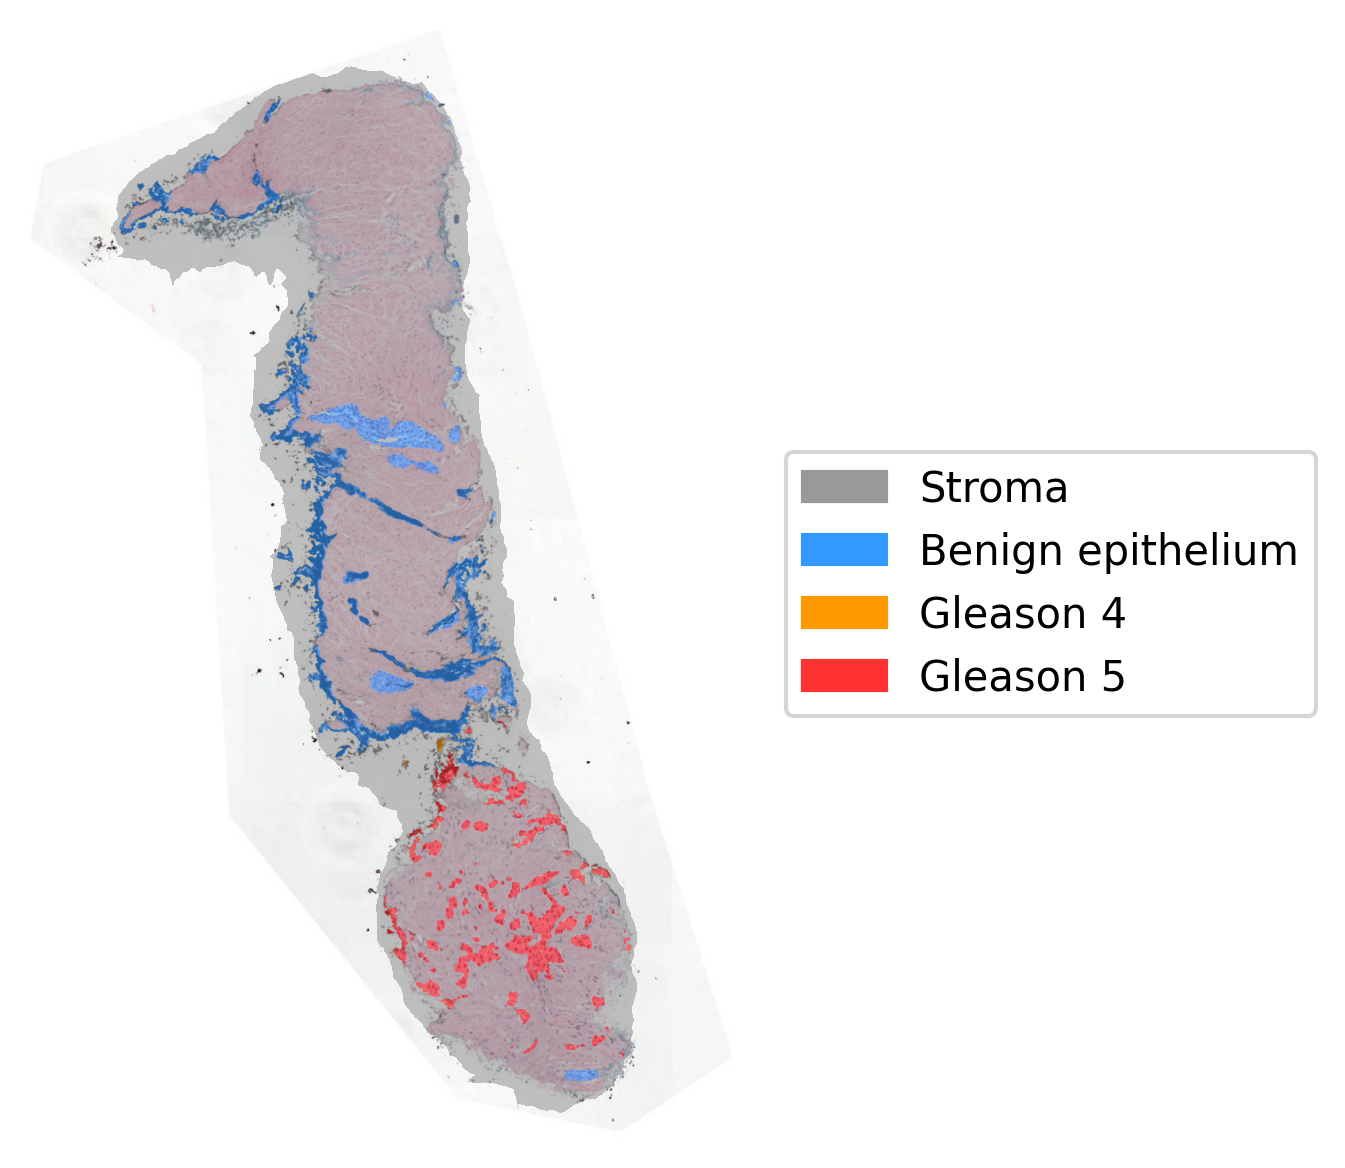
\includegraphics[width=0.8\linewidth]{figuras/mask_discordance}
	\caption{Exemplo de WSI com discordância (ISUP 5 Real vs Predições 0, 3 e 5).}
	\label{fig:mask_discordancia}
\end{figure}

A Figura~\ref{fig:mask_discordancia} mostra o \textit{overlay} da máscara de anotação. Trata-se de uma biópsia longa e fragmentada, com predominância de estroma (cinza) e epitélio benigno (azul), mas contendo áreas malignas significativas: Gleason 4 (laranja) no fragmento superior direito e focos esparsos de Gleason 5 (vermelho) na extremidade inferior direita.  

Do ponto de vista computacional, o modelo B0 apresentou falha na classificação, sugerindo uma limitação na extração de características malignas imersas em tecido estromal denso. O modelo B7, por sua vez, detectou o padrão predominante de Gleason 4, porém não foi capaz de identificar os focos de Gleason 5, culminando em um subestadiamento da amostra para o grau ISUP 3. Em contraste, o B3 foi o único modelo cuja predição refletiu corretamente a conduta de gradação clínica, evidenciando uma maior sensibilidade na detecção de focos esparsos de alta agressividade. Adicionalmente, no que tange às estratégias de ensemble, apenas a regra de agregação pelo valor máximo (\textit{max rule}) foi capaz de consolidar uma predição final correta para este caso.

Este caso evidencia que, em biópsias complexas e fragmentadas, a simples agregação de predições por voto majoritário pode diluir diagnósticos críticos, potencialmente levando a decisões clínicas subótimas. Ressalta-se a importância de estratégias de fusão de modelos mais inteligentes, capazes de ponderar regiões de alto risco e lidar com a heterogeneidade morfológica, além de indicar que a diversidade arquitetural do \textit{ensemble} pode ser explorada para aumentar a robustez diagnóstica.

